\documentclass[]{article}
\usepackage{lmodern}
\usepackage{amssymb,amsmath}
\usepackage{ifxetex,ifluatex}
\usepackage{fixltx2e} % provides \textsubscript
\ifnum 0\ifxetex 1\fi\ifluatex 1\fi=0 % if pdftex
  \usepackage[T1]{fontenc}
  \usepackage[utf8]{inputenc}
\else % if luatex or xelatex
  \ifxetex
    \usepackage{mathspec}
    \usepackage{xltxtra,xunicode}
  \else
    \usepackage{fontspec}
  \fi
  \defaultfontfeatures{Mapping=tex-text,Scale=MatchLowercase}
  \newcommand{\euro}{€}
\fi
% use upquote if available, for straight quotes in verbatim environments
\IfFileExists{upquote.sty}{\usepackage{upquote}}{}
% use microtype if available
\IfFileExists{microtype.sty}{%
\usepackage{microtype}
\UseMicrotypeSet[protrusion]{basicmath} % disable protrusion for tt fonts
}{}
\usepackage[margin=1in]{geometry}
\usepackage{color}
\usepackage{fancyvrb}
\newcommand{\VerbBar}{|}
\newcommand{\VERB}{\Verb[commandchars=\\\{\}]}
\DefineVerbatimEnvironment{Highlighting}{Verbatim}{commandchars=\\\{\}}
% Add ',fontsize=\small' for more characters per line
\usepackage{framed}
\definecolor{shadecolor}{RGB}{248,248,248}
\newenvironment{Shaded}{\begin{snugshade}}{\end{snugshade}}
\newcommand{\KeywordTok}[1]{\textcolor[rgb]{0.13,0.29,0.53}{\textbf{{#1}}}}
\newcommand{\DataTypeTok}[1]{\textcolor[rgb]{0.13,0.29,0.53}{{#1}}}
\newcommand{\DecValTok}[1]{\textcolor[rgb]{0.00,0.00,0.81}{{#1}}}
\newcommand{\BaseNTok}[1]{\textcolor[rgb]{0.00,0.00,0.81}{{#1}}}
\newcommand{\FloatTok}[1]{\textcolor[rgb]{0.00,0.00,0.81}{{#1}}}
\newcommand{\CharTok}[1]{\textcolor[rgb]{0.31,0.60,0.02}{{#1}}}
\newcommand{\StringTok}[1]{\textcolor[rgb]{0.31,0.60,0.02}{{#1}}}
\newcommand{\CommentTok}[1]{\textcolor[rgb]{0.56,0.35,0.01}{\textit{{#1}}}}
\newcommand{\OtherTok}[1]{\textcolor[rgb]{0.56,0.35,0.01}{{#1}}}
\newcommand{\AlertTok}[1]{\textcolor[rgb]{0.94,0.16,0.16}{{#1}}}
\newcommand{\FunctionTok}[1]{\textcolor[rgb]{0.00,0.00,0.00}{{#1}}}
\newcommand{\RegionMarkerTok}[1]{{#1}}
\newcommand{\ErrorTok}[1]{\textbf{{#1}}}
\newcommand{\NormalTok}[1]{{#1}}
\usepackage{graphicx}
\makeatletter
\def\maxwidth{\ifdim\Gin@nat@width>\linewidth\linewidth\else\Gin@nat@width\fi}
\def\maxheight{\ifdim\Gin@nat@height>\textheight\textheight\else\Gin@nat@height\fi}
\makeatother
% Scale images if necessary, so that they will not overflow the page
% margins by default, and it is still possible to overwrite the defaults
% using explicit options in \includegraphics[width, height, ...]{}
\setkeys{Gin}{width=\maxwidth,height=\maxheight,keepaspectratio}
\ifxetex
  \usepackage[setpagesize=false, % page size defined by xetex
              unicode=false, % unicode breaks when used with xetex
              xetex]{hyperref}
\else
  \usepackage[unicode=true]{hyperref}
\fi
\hypersetup{breaklinks=true,
            bookmarks=true,
            pdfauthor={Heather E. Wheeler1,2, GTEx Consortium, Nicholas Knoblauch3, Nancy J. Cox4, Dan L. Nicolae5, Hae Kyung Im5},
            pdftitle={Genetic architecture of gene expression regulation via orthogonal tissue decompositon},
            colorlinks=true,
            citecolor=blue,
            urlcolor=blue,
            linkcolor=magenta,
            pdfborder={0 0 0}}
\urlstyle{same}  % don't use monospace font for urls
\setlength{\parindent}{0pt}
\setlength{\parskip}{6pt plus 2pt minus 1pt}
\setlength{\emergencystretch}{3em}  % prevent overfull lines
\setcounter{secnumdepth}{0}

%%% Use protect on footnotes to avoid problems with footnotes in titles
\let\rmarkdownfootnote\footnote%
\def\footnote{\protect\rmarkdownfootnote}

%%% Change title format to be more compact
\usepackage{titling}

% Create subtitle command for use in maketitle
\newcommand{\subtitle}[1]{
  \posttitle{
    \begin{center}\large#1\end{center}
    }
}

\setlength{\droptitle}{-2em}
  \title{Genetic architecture of gene expression regulation via orthogonal tissue
decompositon}
  \pretitle{\vspace{\droptitle}\centering\huge}
  \posttitle{\par}
  \author{Heather E. Wheeler\textsuperscript{1,2}, GTEx Consortium, Nicholas
Knoblauch\textsuperscript{3}, Nancy J. Cox\textsuperscript{4}, Dan L.
Nicolae\textsuperscript{5}, Hae Kyung Im\textsuperscript{5}}
  \preauthor{\centering\large\emph}
  \postauthor{\par}
  \predate{\centering\large\emph}
  \postdate{\par}
  \date{2015-09-03 16:49:21 \textsuperscript{1}Department of Biology and
\textsuperscript{2}Department of Computer Science, Loyola University
Chicago, \textsuperscript{3}Committee on Genetics, Genomics, and Systems
Biology, University of Chicago, \textsuperscript{4}Division of Genetic
Medicine, Vanderbilt University, \textsuperscript{5}Section of Genetic
Medicine, Department of Medicine, University of Chicago}



\begin{document}

\maketitle


\section{Abstract}\label{abstract}

For many complex traits, gene regulation is likely to play a crucial
mechanistic role given the consistent enrichment of expression
quantitative trait loci (eQTLs) among trait-associated variants. In
order to fully harness gene regulation mechanisms in future studies of
complex traits, we sought to better understand the underlying genetic
architecture of the gene regulation traits themselves. We show that
local heritability of gene expression (variance in gene expression due
to genetic variation within 1Mb of a gene) can be accurately estimated
across tissues, but distal heritability cannot be reliably estimated at
sample sizes less than 1000. Using both the elastic net and Bayesian
sparse linear mixed modeling, we show that for local gene regulation,
the genetic architecture is mostly sparse rather than polygenic. Using
genome and transcriptome data from the diverse set of tissues available
in The GTEx Project, we developed a model called Orthogonal Tissue
Decomposition (OTD), which partitions gene expression into cross-tissue
and tissue-specific components. Estimates of the local heritability of
OTD-generated cross-tissue gene expression have larger magnitude and
smaller standard errors compared to single tissue estimates due to the
borrowing of information across all samples. We show that genes with
high cross-tissue heritability are more likely to have cross-tissue
eQTLs, confirming that OTD is capturing the cross-tissue component of
gene expression. We also found evidence that genes with large
tissue-specific heritability are enriched in common complex disease
genes discovered via GWAS. Cross-validated predictors of cross-tissue
and tissue-specific expression built here have been added to the
PrediXcan database for future investigations of complex traits.

\section{Introduction}\label{introduction}

Regulatory variation has been shown to play a key role in the genetics
of complex traits {[}1--3{]}. While many common diseases have been shown
to be polygenic {[}4--6{]}, it is unclear whether gene expression levels
are also polygenic or instead have simpler genetic architectures and how
much these expression architectures vary across genes {[}7{]}. Most
human expression quantitative trait loci (eQTL) studies have focused on
how local genetic variation affects gene expression in order to reduce
the multiple testing burden that would be required for a global analysis
{[}7,8{]}. Furthermore, when both local and distal eQTLs are reported
{[}9--11{]}, effect sizes and replicability are much higher for local
eQTLs. Indeed, while the heritability of gene expression attributable to
local genetic variation has been estimated accurately, large standard
errors have prevented accurate estimation of the contribution of distal
genetic variation to gene expression variation {[}11,12{]}.

Most human eQTL studies have been performed in whole blood or
lymphoblastoid cell lines due to ease of access or culturabilty
{[}9,13,14{]}. The Genotype-Tissue Expression (GTEx) Project aims to
examine the genetics of gene expression more comprehensively and
recently published a pilot analysis of RNA sequencing data from 1641
samples across 43 tissues from 175 individuals {[}15{]}. In order to
better understand the genetic architecture of tissue-specific and
cross-tissue gene regulation, we developed a mixed effects model called
orthogonal tissue decomposition (OTD) to determine the cross-tissue and
tissue-specific components of gene expression in the rich GTEx dataset.
These components were used to develop predcitors of cross-tissue and
tissue-specific gene expression for use in our gene-based association
method PrediXcan {[}16{]}.

We also assessed the ability of various models with different underlying
assumptions to predict gene expression in order to understand the
underlying genetic architecture of gene expression. Gene expression
traits with sparse architecture should be better predicted with sparse
models such as LASSO (Least Absolute Shrinkage and Selection Operator)
{[}17{]} while highly polygenic traits should be better predicted with
ridge regression or similarly polygenic models {[}18--20{]}. Using the
hybrid approach of BSLMM (Bayesian Sparse Linear Mixed Model) {[}21{]},
we quantified the proportion of the sparse component that makes up the
total proportion of expression variance explained by sparse and
polygenic effects.

Specifically, in this paper we show that local heritability can be
accurately estimated across tissues, but distal heritability cannot
reliably estimated at current sample sizes. We also show that for local
gene regulation, the genetic architecture is mostly sparse rather than
polygenic. We found that estimates of the local heritability of
cross-tissue gene expression generated with our OTD model have larger
magnitude and improved standard errors compared to single tissue
estimates due to the borrowing of information across all samples.
Comparing our OTD results to a previously performed joint multi-tissue
eQTL analysis method {[}22{]}, we show that genes with high cross-tissue
heritability are more likely to have cross-tissue eQTLs, confirming that
OTD is capturing the cross-tissue component of gene expression. We also
found evidence that genes with large tissue-specific heritability are
enriched in common complex disease genes discovered via GWAS. {[}{[}Redo
with PVE estimates from BSLMM{]}{]}

\section{Results}\label{results}

\subsection{Local genetic variation explains a large proportion of gene
expression
variance}\label{local-genetic-variation-explains-a-large-proportion-of-gene-expression-variance}

We estimated the heritability of gene expression in whole blood from the
Depression Genes and Networks (DGN) cohort (n=922) {[}14{]} using a
mixed-effects model (see Methods) and calculated variances using
restricted maximum likelihood as implemented in GCTA {[}23{]}. We fit a
joint model with a local and a distal genetic relationship matrix (GRM).
The local GRM was derived from SNPs within 1 Mb of each gene and the
distal GRM was derived from SNPs that are located on non-gene
chromosomes and are eQTLs in the Framingham Heart Study (FHS) cohort
(n=5257, FDR \textless{} 0.05) {[}24{]}. The mean local
h\textsuperscript{2} was 0.130 and 54.6\% of genes had a positive 95\%
confidence interval (CI), while the mean distal h\textsuperscript{2} was
0.076 and just 4.2\% of genes had a positive CI (Fig 1). The maximum
local h\textsuperscript{2} was 0.93 with a standard error (SE) of 0.009
while the maximum distal h\textsuperscript{2} was 0.91 with a SE of
0.16. Similar results were observed for the 1194 genes with
\emph{trans}-eQTLs (FHS FDR \textless{} 0.05) when the distal GRM was
limited to known \emph{trans}-eQTLs (Fig 2). That is, the mean local
h\textsuperscript{2} was 0.133 and 61.3\% of genes had a positive 95\%
confidence interval (CI), while the mean \emph{trans}
h\textsuperscript{2} was just 0.021 and 4.2\% of genes tested had a
positive CI.

\subsection{The effect of local genetic variation on gene expression is
sparse rather than
polygenic}\label{the-effect-of-local-genetic-variation-on-gene-expression-is-sparse-rather-than-polygenic}

We performed 10-fold cross-validation using the elastic net {[}25{]} to
test the predictive performance of local SNPs for gene expression across
a range of mixing parameters, \(\alpha\). The \(\alpha\) that gives the
largest cross-validation R\textsuperscript{2} informs the sparsity of
each gene expression trait. That is, at one extreme, if the optimal
\(\alpha=0\) (equivalent to ridge regression), the gene expression trait
is highly polygenic, whereas if the optimal \(\alpha=1\) (equivalent to
LASSO), the trait is highly sparse. We found that for most gene
expression traits, the cross-validated R\textsuperscript{2} was
suboptimal for \(\alpha=0\) and \(\alpha=0.05\), but nearly identically
optimal for \(\alpha=0.5\) and \(\alpha=1\) in the DGN cohort (Fig 3).
This suggests that for most genes, the effect of local genetic variation
on gene expression is sparse rather than polygenic.

To further examine sparsity and polygenicity, we used BSLMM {[}21{]} to
define the total proportion of variance in expression explained by
sparse and polygenic effects together (PVE) and the proportion of this
genetic variance explained by sparse effects (PGE) for each gene in the
DGN cohort. The PVE can be thought of as a Bayesian estimate of chip
heritability and, indeed, there is a strong correlation between
BSLMM-estimated PVE and GCTA-estimated h\textsuperscript{2} (Fig 4A,
R=0.96). For genes with large PVE, the PGE also was large, indicative of
a sparse genetic architecture. For example, all genes with PVE
\textgreater{} 0.50 had PGE \textgreater{} 0.82 and their median PGE was
0.989 (Fig 4B). The median PGE for genes with PVE \textgreater{} 0.1 was
0.949. Fittingly, for most (96.3\%) of the genes with PVE estimates
\textgreater{} 0.10, the median number of SNPs included in the model was
no more than 10 (Fig 4C).

\subsection{Cross-tissue and tissue-specific gene expression by
orthogonal tissue
decomposition}\label{cross-tissue-and-tissue-specific-gene-expression-by-orthogonal-tissue-decomposition}

In order to better understand the context specificity of gene expression
regulation, we developed a method called orthogonal tissue decomposition
(OTD), which uses a mixed effects model to generate cross-tissue and
tissue-specific gene expression levels (see Methods). Using a marginal
model with just the local GRM, we estimated the local
h\textsuperscript{2} of cross-tissue gene expression and tissue-specific
gene expression in the nine tissues with the most samples. The
cross-tissue heritabilities were larger and the standard errors were
smaller than the tissue-specific estimates (Fig 5). The percentage of
h\textsuperscript{2} estimates with positive CIs was much larger for
cross-tissue expression (17.3\%) than the tissue-specific expressions
(all less than 3\%, Fig 6).

We also compared the cross-tissue h\textsuperscript{2} from the OTD to
h\textsuperscript{2} estimates from the pre-OTD measures of gene
expression in each of the nine tissues, which we term tissue-wide
expression. Again, the cross-tissue heritabilities were larger and the
standard errors were smaller than the tissue-wide estimates (Fig 7),
though less striking than the tissue-specific comparison. The percentage
of tissue-wide h\textsuperscript{2} estimates with positive CIs ranged
from 4.4-8.6\% and thus were all larger than the tissue-specific postive
CI percentages, but smaller than the cross-tissue percentage (Fig 8).

We compared our OTD results to those from a joint multi-tissue eQTL
analysis method {[}22{]}, which was previously performed on a subset of
the GTEx data {[}15{]}. The results of this analysis include eQTL
posterior probabilities for each of the nine tissues, which can be
interpreted as the probability a SNP is an eQTL in tissue \emph{x} given
the data. Using the top eQTL for each gene, we defined an entropy
statistic (see Methods) that combines the nine posterior probabilities
into one value such that higher entropy values mean the gene is more
likely to be regulated by the same eQTL across all nine tissues, rather
than in just a subset of the nine. We observed a strong correlation
between entropy and both the cross-tissue expression heritability (R =
0.082, Fig 9A) and PVE (R = 0.12, Fig 9B) estimates, using the
cross-tissue expression derived from the OTD. Thus, genes with high
cross-tissue heritability are more likely to have cross-tissue eQTLs,
confirming that OTD is capturing the cross-tissue component of gene
expression. Also, the correlation between tissue-specific OTD gene
expression PVE and the posterior probability that the gene has an eQTL
in that tissue is strongest in each respective tissue, confirming that
OTD also captures tissue-specific components of gene expression (Fig
10).

\section{Discussion}\label{discussion}

Because regulatory variation plays a key mechanistic role in the
genetics of complex traits {[}1--3{]}, we sought to comprehensively
characterize the genetic architecture of gene expression across tissues.
We show that the local architecture of gene expression is sparse for
95\% of heritable genes and that distal architecture cannot be accrately
assessed at current sample sizes (n \textless{} 1000). {[}{[}compare
mean h2's across studies{]}{]} Indeed, while the heritability of gene
expression attributable to local genetic variation has been estimated
accurately, large standard errors have prevented accurate estimation of
the contribution of distal genetic variation to gene expression
variation {[}11,12{]}.

We developed a mixed effects model called orthogonal tissue
decomposition (OTD) to determine the cross-tissue and tissue-specific
components of gene expression in the rich GTEx dataset. These components
were used to develop predcitors of cross-tissue and tissue-specific gene
expression for use in our gene-based association method PrediXcan
{[}16{]}. The tissue availability is unbalanced because of the
difficulties of sample collection and the uneven quality of the tissues.
Furthermore, by using a mixed effects model to create cross-tissue
expression, we borrow information across tissues, which should increase
our power to detect associations and achieve better predictive models.

We also assessed the ability of various models with different underlying
assumptions to predict gene expression in order to understand the
underlying genetic architecture of gene expression. Gene expression
traits with sparse architecture should be better predicted with sparse
models such as LASSO (Least Absolute Shrinkage and Selection Operator)
{[}17{]} while highly polygenic traits should be better predicted with
ridge regression or similarly polygenic models {[}18--20{]}. Using the
hybrid approach of BSLMM (Bayesian Sparse Linear Mixed Model) {[}21{]},
we quantified the proportion of the sparse component that makes up the
total proportion of expression variance explained by sparse and
polygenic effects.

Specifically, in this paper we show that local heritability can be
accurately estimated across tissues, but distal heritability cannot
reliably estimated at current sample sizes. We also show that for local
gene regulation, the genetic architecture is mostly sparse rather than
polygenic. We found that estimates of the local heritability of
cross-tissue gene expression generated with our OTD model have larger
magnitude and improved standard errors compared to single tissue
estimates due to the borrowing of information across all samples.
Comparing our OTD results to a previously performed joint multi-tissue
eQTL analysis method {[}22{]}, we show that genes with high cross-tissue
heritability are more likely to have cross-tissue eQTLs, confirming that
OTD is capturing the cross-tissue component of gene expression.

\begin{enumerate}
\def\labelenumi{\arabic{enumi}.}
\itemsep1pt\parskip0pt\parsep0pt
\item
  local + trans heritability (others have done this)
\item
  trans heritability estimates not reliable, proportion not reliable
\item
  orthogonal tissue decomposition
\item
  cross tissue + tissue specific heritability -- estimates higher and se
  lower for cross-tissue The tissue availability is unbalanced because
  of the difficulties of sample collection and the uneven quality of the
  tissues. Furthermore, by using a mixed effects model to create
  cross-tissue expression, we borrow information across tissues, which
  should increase our power to detect associations and achieve better
  predictive models.
\item
  elastic net mixing parameter (alpha) as measure of
  polygenicity/sparsity
\end{enumerate}

Future

\begin{enumerate}
\def\labelenumi{\arabic{enumi}.}
\itemsep1pt\parskip0pt\parsep0pt
\item
  simulation to show sparsity well represented by alpha
\item
  use number of PC's (computed using only local snps) that maximize
  prediction performance. This will count independent signals.
\item
  FHS heritability. could this improve trans heritability?
\end{enumerate}

\section{Methods}\label{methods}

\subsection{Genomic and Transcriptomic
Data}\label{genomic-and-transcriptomic-data}

\subsubsection{DGN Dataset}\label{dgn-dataset}

We obtained whole blood RNA-Seq and genome-wide genotype data for 922
individuals from the Depression Genes and Networks (DGN) cohort
{[}14{]}, all of European ancestry. For our analyses, we used the HCP
(hidden covariates with prior) normalized gene-level expression data
used for the \emph{trans}-eQTL analysis in Battle et al. {[}14{]} and
downloaded from the NIMH repository. The 922 individuals were unrelated
(all pairwise \(\hat{\pi}\) \textless{} 0.05) and thus all included in
downstream analyses. Imputation of approximately 650K input SNPs (minor
allele frequency {[}MAF{]} \textgreater{} 0.05, Hardy-Weinberg
Equilibrium {[}P \textgreater{} 0.05{]}, non-ambiguous strand {[}no A/T
or C/G SNPs{]}) was performed on the University of Michigan
Imputation-Server
(\url{https://imputationserver.sph.umich.edu/start.html}) {[}26,27{]}
with the following parameters: 1000G Phase 1 v3 ShapeIt2 (no singletons)
reference panel, SHAPEIT phasing, and EUR population. Approximately 1.9M
non-ambiguous strand SNPs with MAF \textgreater{} 0.05, imputation
R\textsuperscript{2} \textgreater{} 0.8 and, to reduce computational
burden, inclusion in HapMap Phase II were retained for subsequent
analyses.

\subsubsection{GTEx Dataset}\label{gtex-dataset}

We obtained RNA-Seq gene expression levels from 8555 tissue samples (53
unique tissue types) from 544 unique subjects in the GTEx Project
{[}15{]} data release on 2014-06-13. Of the individuals with gene
expression data, genome-wide genotypes (imputed with 1000 Genomes) were
available for 450 individuals. While all 8555 tissue samples were used
in the OTD model (described below) to generate cross-tissue and
tissue-specific components of gene expression, we used the nine tissues
with the largest sample sizes when quantifying tissue-specific effects.
Tissues and sample sizes (both RNA-seq and genotypes available) included
cross-tissue (\(n=450\)), skeletal muscle (\(n=361\)), whole blood
(\(n=339\), skin from the sun-exposed portion of the lower leg
(\(n=303\)), subcutaneous adipose (\(n=298\)), tibial artery
(\(n=285\)), lung (\(n=279\)), thyroid (\(n=279\)), tibial nerve
(\(n=256\)) and left ventricle heart (\(n=190\)). Approximately 2.6M
non-ambiguous strand SNPs included in HapMap Phase II were retained for
subsequent analyses.

\subsection{Partitioning local and distal heritability of gene
expression}\label{partitioning-local-and-distal-heritability-of-gene-expression}

To investigate the proximity of gene expression regulation to each gene,
we partitioned the proportion of gene expression variance explained by
SNPs in the DGN cohort into two components: local (SNPs within 1Mb of
the gene) and distal (eQTLs on non-gene chromosomes) as defined by the
GENCODE {[}28{]} version 12 gene annotation. We calculated the
proportion of the variance (narrow-sense heritability) explained by each
component using the following mixed-effects model:

\[ Y_g = \sum_{k = \in local}w_{k,g} X_k + \sum_{k = \in distal}w_{k,g} X_k + \epsilon \]

Assuming a random effects for \(w_{k,g} \approx N(0, \sigma^2_w)\) and
\(\epsilon \approx N(0, \sigma^2_{\epsilon} I_n)\), where \(I_n\) is the
identity matrix, we calculated the total variability explained by local
and distal components by estimating \(\sigma^2_w\) with restricted
maximum likelihood (REML) using GCTA software {[}23{]}. For heritability
analyses in the GTEx cohort, we removed the \(distal\) term from the
model and only estimated marginal \(local\) h\textsuperscript{2} due to
the smaller sample sizes of both cross-tissue and tissue-specific
expression levels compared to DGN.

\subsection{Determining polygenicity versus sparsity using the elastic
net}\label{determining-polygenicity-versus-sparsity-using-the-elastic-net}

We applied the elastic net {[}25{]} to model the effect of local genetic
variation (SNPs within 1 Mb of gene) on the genetic architecture of gene
expression. We used the \texttt{cv.glmnet} function in the R package
\texttt{glmnet} {[}29,30{]} to perform 10-fold cross-validation of the
elastic net across a range of mixing paramaters (\(\alpha\)) to find the
\(\alpha\) that maximized predictive performance, measured by Pearson's
R\textsuperscript{2}. Specifically, \texttt{glmnet} solves the following
problem:

\textbf{{[}{[}Haky, should/can we simplify this equation? I just took it
from \url{http://web.stanford.edu/~hastie/glmnet/glmnet_alpha.html}, but
they don't explain all the terms{]}{]}}
{\[\min_{\beta_0,\beta} \frac{1}{N} \sum_{i=1}^{N} w_i l(y_i,\beta_0+\beta^T x_i) + \lambda\left[(1-\alpha)||\beta||_2^2/2 + \alpha ||\beta||_1\right], \]}

over a grid of values of \(\lambda\) covering the entire range
{[}29,30{]}. This tuning parameter \(\lambda\) controls the overall
strength of the penalty.

The elastic net penalty is controlled by mixing parameter \(\alpha\),
which spans LASSO (\(\alpha=1\), the default) {[}17{]} at one extreme
and ridge regression (\(\alpha=0\)) {[}18{]} at the other. The ridge
penalty shrinks the coefficients of correlated SNPs towards each other,
while the LASSO tends to pick one of the correlated SNPs and discard the
others. Thus, an optimal prediction R\textsuperscript{2} for
\(\alpha=0\) means the gene expression trait is highly polygenic, while
an optimal prediction R\textsuperscript{2} for \(\alpha=1\) means the
trait is highly sparse. An optimal prediction R\textsuperscript{2} in
between (e.g. \(\alpha=0.5\)) means the trait has a mixed genetic
architecture.

In the DGN cohort, we tested 21 values of the mixing parameter
(\(\alpha=0, 0.05, 0.1, ..., 0.90, 0.95, 1\)) for optimal prediction of
gene expression of the 341 genes on chromosome 22. For the rest of the
autosomes in DGN and for cross-tissue, tissue-specific, and tissue-wide
expression in the GTEx cohort, we tested \(\alpha=0.05, 0.5, 0.95, 1\).
\textbf{{[}{[}add when finished, need to do DGN alpha=0.05 and
0.95{]}{]}}

\subsection{Quantifying sparsity with Bayesian Sparse Linear Mixed
Models
(BSLMM)}\label{quantifying-sparsity-with-bayesian-sparse-linear-mixed-models-bslmm}

We used BSLMM {[}21{]} to model the effect of local genetic variation
(SNPs within 1 Mb of gene) on the genetic architecture of gene
expression. The BSLMM consists of a standard linear mixed model, with
one random effect term, and with sparsity inducing priors on the
regression coefficients {[}21{]}. We used the software GEMMA {[}31{]} to
implement BSLMM for each gene using the following parameters:

\begin{Shaded}
\begin{Highlighting}[]
\NormalTok{gemma -g [localGenoFile] -p [geneExpFile] -a [snpAnnotFile] -bslmm }\DecValTok{1} \NormalTok{-s }\DecValTok{100000} \NormalTok{-o [outFile]}
\end{Highlighting}
\end{Shaded}

The \texttt{-bslmm 1} option specifies a linear BSLMM and the
\texttt{-s 100000} option specifies the number of sampling steps per
gene. The BSLMM estimates the PVE (the total proportion of variance in
phenotype explained by the sparse effects and random effects terms
together) and PGE (the proportion of genetic variance explained by the
sparse effects terms). From the second half of the sampling iterations
for each gene, we report the median and the 95\% credible sets of the
PVE, PGE, and the \textbar{}\(\gamma\)\textbar{} parameter (the number
of SNPs with non-zero coefficients).

\subsection{Orthogonal tissue
decomposition}\label{orthogonal-tissue-decomposition}

To better understand the context specificity of gene expression
regulation, we developed a method called orthogonal tissue decomposition
(OTD). This approach is an extension of our method to develop an
intrinsic growth phenotype {[}32{]}. We applied OTD to GTEx Project
{[}15{]} data and decomposed the expression of each gene into
cross-tissue and tissue-specific components. The tissue availability is
unbalanced across individuals because of the difficulties of sample
collection and the uneven quality of the tissues. OTD decomposes the
expression traits into orthogonal components as represented by the
following model:

\[ Y_i = T_{i,cross} + T_{i,tissue} \]

Specifically, to generate cross-tissue and tissue-specific expression
levels, we used the \texttt{lmer} function in the R {[}33{]} package
\texttt{lme4} {[}34,35{]} to fit the following mixed-effects model:

\begin{Shaded}
\begin{Highlighting}[]
\NormalTok{fit <-}\StringTok{ }\NormalTok{lme4::}\KeywordTok{lmer}\NormalTok{(expression ~}\StringTok{ }\NormalTok{(}\DecValTok{1}\NormalTok{|SUBJID) +}\StringTok{ }\NormalTok{TISSUE +}\StringTok{ }\NormalTok{GENDER +}\StringTok{ }\NormalTok{PEERs)}
\end{Highlighting}
\end{Shaded}

The model included tissue-wide gene expression levels in 8555 GTEx
tissue samples from 544 unique subjects. A total of 17,647
Protein-coding genes (defined by GENCODE {[}28{]} version 18) with a
mean gene expression level across tissues greater than 0.1 RPKM (reads
per kilobase of transcript per million reads mapped) were included in
the model. \texttt{SUBJID} was a random effect and the covariates
\texttt{TISSUE}, \texttt{GENDER}, and \texttt{PEERs} were fixed effects
used to predict tissue-wide expression levels (\texttt{expression} in
the model). \texttt{PEERs} included the top 15 PEER factors estimated
across all tissues using the R package \texttt{PEER} {[}36{]} to control
for batch effects and experimental confounders. Cross-tissue expression
was defined as the random effects from the model (\texttt{ranef(fit)})
and tissue-specific expression as the residuals (\texttt{resid(fit})).

\subsection{Comparison of OTD PVE to multi-tissue eQTL
results}\label{comparison-of-otd-pve-to-multi-tissue-eqtl-results}

Using results from a joint multi-tissue eQTL analysis method {[}22{]}
performed with a subset of the GTEx data (maximum n=175 in the nine
tissues of the pilot phase, see {[}15{]}), we defined an entropy
statistic to compare these results to those from our OTD method. The
results of the multi-tissue analysis include eQTL posterior
probabilities for each of the nine tissues, which can be interpreted as
the probability a SNP is an eQTL in tissue \(t\) given the data. Using
the top eQTL for each gene \(g\), we defined the entropy \(S_g\) as:

\[ S_g = -\sum_{t}p_{t,g} \log p_{t,g} \]

where \(p_{t,g}\) is the eQTL probability in tissue \(t\) normalized to
1 for each gene \(g\). Thus, eQTLs with higher entropy statistics are
more likely to be cross-tissue eQTLs, rather than only regulating gene
expression in one or a few tissues. We calculated the Pearson
correlation between \(S_g\) and the cross-tissue expression heritability
and PVE for each gene to verify that our OTD method captures
cross-tissue effects. We also calculated a Pearson correlation matrix
between the posterior probabilities in each tissue from the multi-tissue
eQTL method and the tissue-specific gene expression PVE from the OTD
method.

\subsection{Enrichment analysis}\label{enrichment-analysis}

\begin{itemize}
\itemsep1pt\parskip0pt\parsep0pt
\item
  For top CT and TS genes:
\end{itemize}

\begin{enumerate}
\def\labelenumi{\arabic{enumi}.}
\itemsep1pt\parskip0pt\parsep0pt
\item
  GO enrichment
\item
  GWAS catalog enrichment (i.e.~top T2D, T1D, schizo, etc. genes)
  {[}{[}redo GWAS catalog enrichment with CT and TS top PVE{]}{]}
\end{enumerate}

\subsection{Tables}\label{tables}

\section{Figures}\label{figures}

\begin{figure}[htbp]
\centering
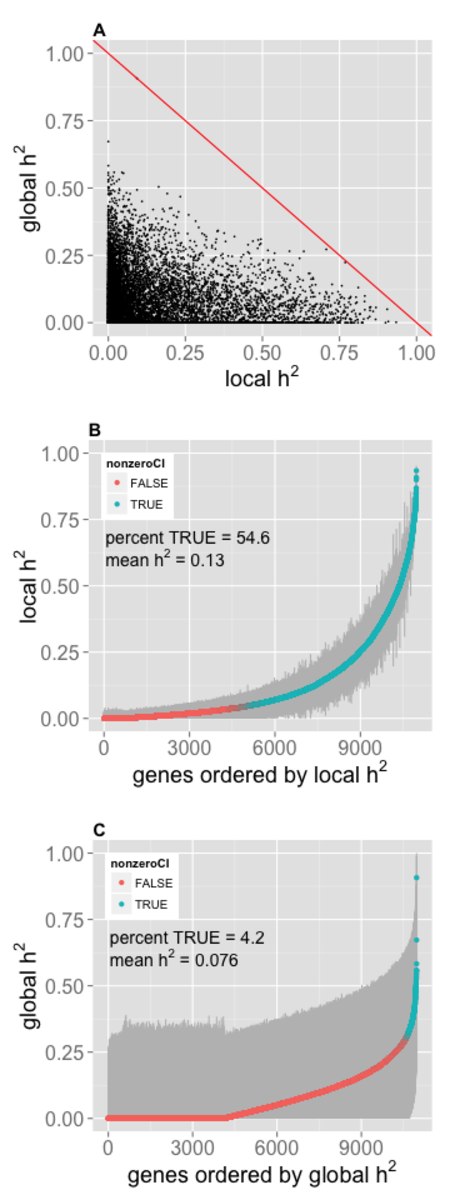
\includegraphics{GenArch_manuscript_files/figure-latex/jointH2-1.pdf}
\caption{DGN whole blood expression joint heritability
(h\textsuperscript{2}). Local (SNPs within 1 Mb of each gene) and distal
(SNPs that are eQTLs in the Framingham Heart Study on other chromosomes
{[}FDR \textless{} 0.05{]}) h\textsuperscript{2} for gene expression
were jointly estimated. (\textbf{A}) Distal h\textsuperscript{2}
compared to local h\textsuperscript{2} per gene. (\textbf{B}) Local and
(\textbf{C}) distal gene expression h\textsuperscript{2} estimates
ordered by increasing h\textsuperscript{2}. The 95\% confidence interval
(CI) of each h\textsuperscript{2} estimate is in gray and genes with a
lower bound greater than zero are in blue.}
\end{figure}

\begin{figure}[htbp]
\centering
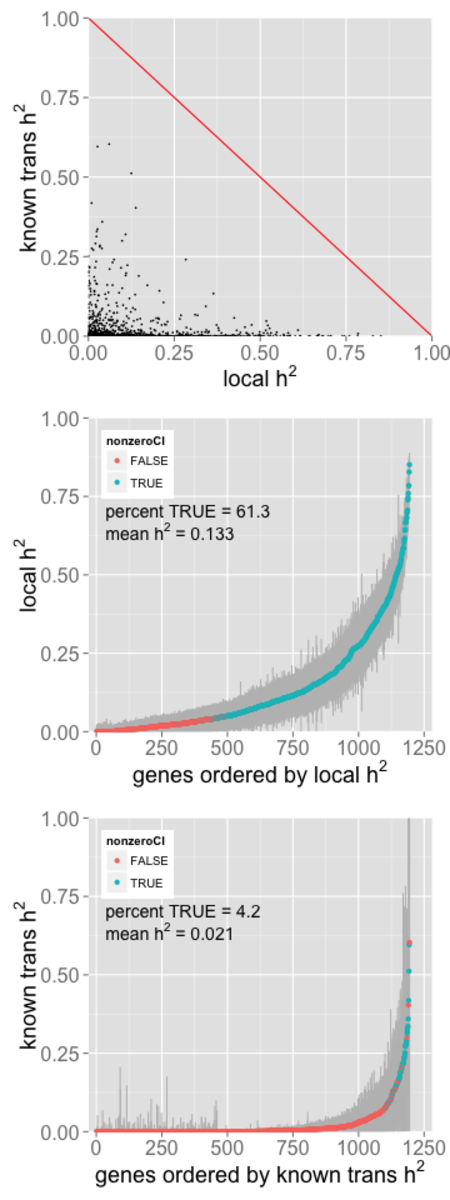
\includegraphics{GenArch_manuscript_files/figure-latex/transH2-1.pdf}
\caption{DGN whole blood expression joint heritability
(h\textsuperscript{2}) with known trans-eQTLs. Local (SNPs within 1 Mb
of each gene) and known trans (SNPs that are trans-eQTLs in the
Framingham Heart Study for each gene {[}FDR \textless{} 0.05{]})
h\textsuperscript{2} for gene expression were jointly estimated.
(\textbf{A}) Known trans h\textsuperscript{2} compared to local
h\textsuperscript{2} per gene. (\textbf{B}) Local and (\textbf{C}) known
trans gene expression h\textsuperscript{2} estimates ordered by
increasing h\textsuperscript{2}. The 95\% confidence interval (CI) of
each h\textsuperscript{2} estimate is in gray and genes with a lower
bound greater than zero are in blue.}
\end{figure}

\begin{figure}[htbp]
\centering
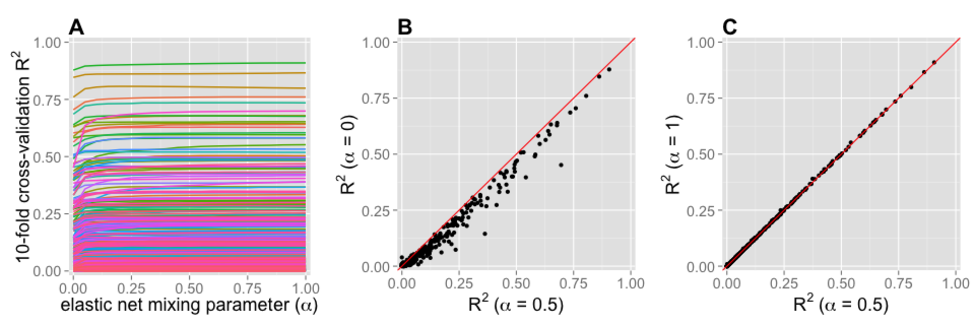
\includegraphics{GenArch_manuscript_files/figure-latex/EN-1.pdf}
\caption{Cross-validated predictive performance across the elastic net.
(\textbf{A}) 10-fold cross-validated R\textsuperscript{2} of predicted
vs.~observed expression in DGN whole blood compared to a range of
elastic net mixing parameters (\(\alpha\)) for genes on chromosome 22
with R\textsuperscript{2} \textgreater{} 0.3. (\textbf{B}) Predictive
R\textsuperscript{2} difference between LASSO (\(\alpha = 1\)) and
several other values of \(\alpha\) compared to LASSO predictive
R\textsuperscript{2} for 341 genes on chromosome 22.}
\end{figure}

\begin{figure}[htbp]
\centering
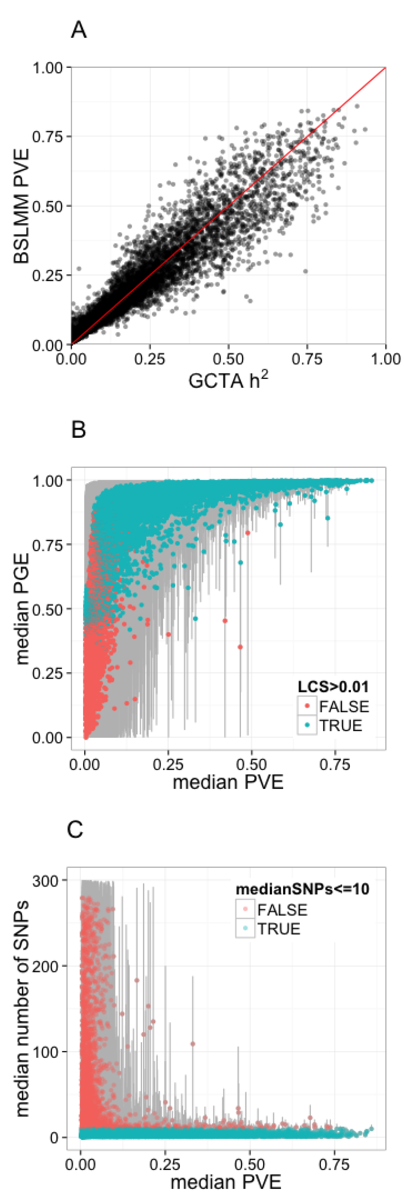
\includegraphics{GenArch_manuscript_files/figure-latex/dgnBSLMM-1.pdf}
\caption{Bayesian Sparse Linear Mixed Models reveal the sparsity of gene
expression architecture. (\textbf{A}) BSLMM-estimated PVE (total
proportion of variance explained) compared to GCTA-estimated
heritability per gene (R=0.96) (\textbf{B}) Comparison of median PGE
(proportion of PVE explained by sparse effects) to median PVE (total
proportion of variance explained) for expression of each gene. The 95\%
credible set of each PGE estimate is in gray and genes with a lower
credible set (LCS) greater than 0.01 are in blue. (\textbf{C})
Comparison of the median number of SNPs included in the model of each
gene to median PVE. The 95\% credible set of each SNP-number estimate is
in gray and genes with a median of 10 or fewer SNPs are in blue.}
\end{figure}

\begin{figure}[htbp]
\centering
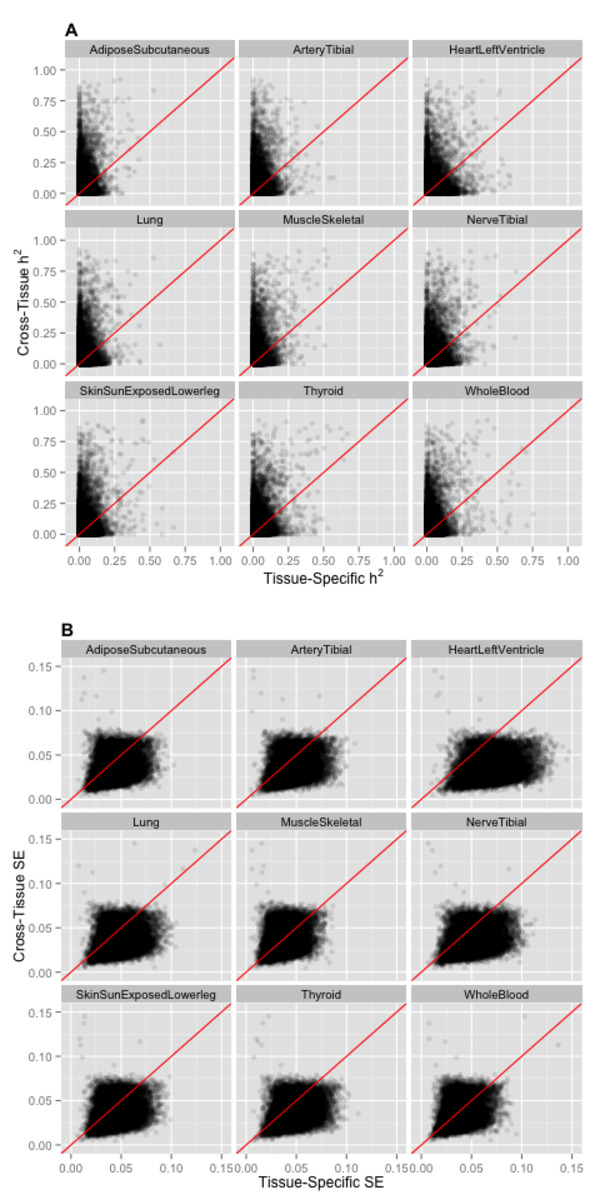
\includegraphics{GenArch_manuscript_files/figure-latex/TSotdH2SE-1.pdf}
\caption{Cross-tissue and tissue-specific comparison of heritability
(h\textsuperscript{2}, \textbf{A}) and standard error (SE, \textbf{B})
estimation. Cross-tissue local h\textsuperscript{2} is estimated using
the cross-tissue component (random effects) of the mixed effects model
for gene expression and SNPs within 1 Mb of each gene. Tissue-specifc
local h\textsuperscript{2} is estimated using the tissue-specific
component (residuals) of the mixed effects model for gene expression for
each respective tissue and SNPs within 1 Mb of each gene.}
\end{figure}

\begin{figure}[htbp]
\centering
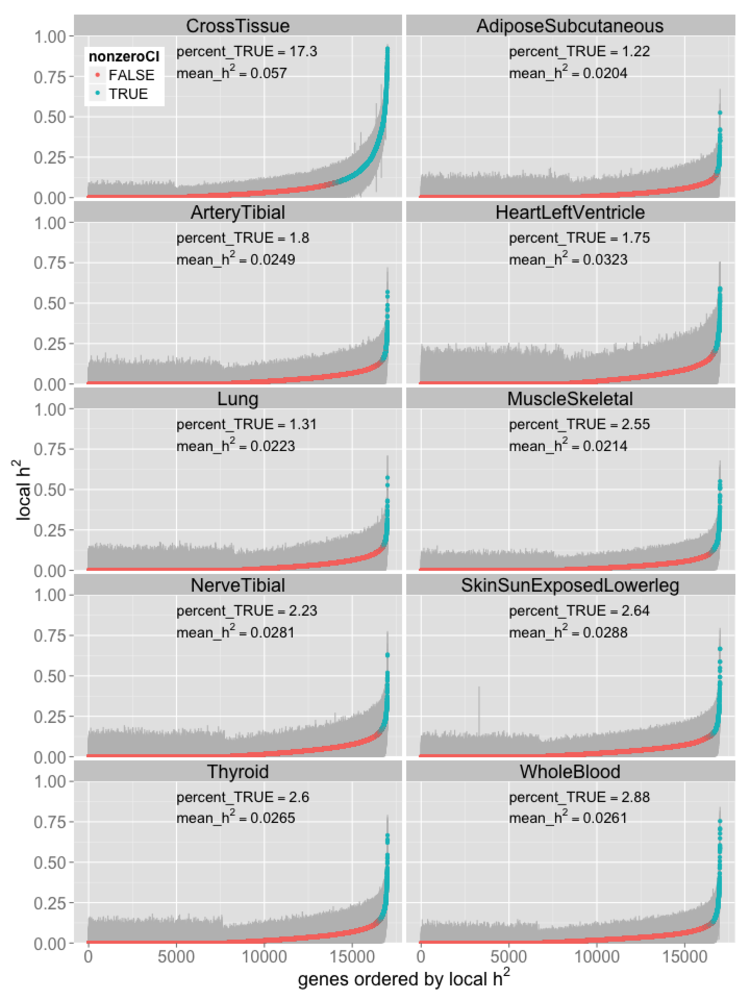
\includegraphics{GenArch_manuscript_files/figure-latex/otdTSh2-1.pdf}
\caption{Cross-tissue heritability (h\textsuperscript{2}) compared to
tissue-specific h\textsuperscript{2}. Cross-tissue local
h\textsuperscript{2} is estimated using the cross-tissue component
(random effects) of the mixed effects model for gene expression and SNPs
within 1 Mb of each gene. Tissue-specifc local h\textsuperscript{2} is
estimated using the tissue-specific component (residuals) of the mixed
effects model for gene expression for each respective tissue and SNPs
within 1 Mb of each gene.}
\end{figure}

\begin{figure}[htbp]
\centering
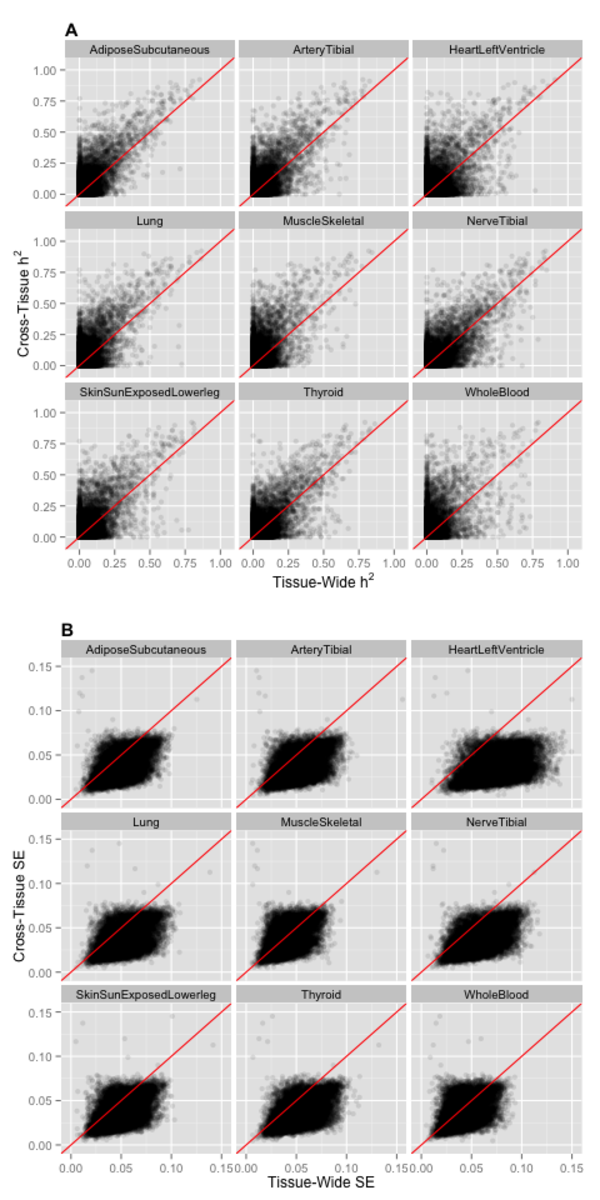
\includegraphics{GenArch_manuscript_files/figure-latex/TWotdH2SE-1.pdf}
\caption{Cross-tissue and tissue-wide comparison of heritability
(h\textsuperscript{2}, \textbf{A}) and standard error (SE, \textbf{B}).
Cross-tissue local h\textsuperscript{2} is estimated using the
cross-tissue component (random effects) of the mixed effects model for
gene expression and SNPs within 1 Mb of each gene. Tissue-wide local
h\textsuperscript{2} is estimated using the measured gene expression for
each respective tissue and SNPs within 1 Mb of each gene.}
\end{figure}

\begin{figure}[htbp]
\centering
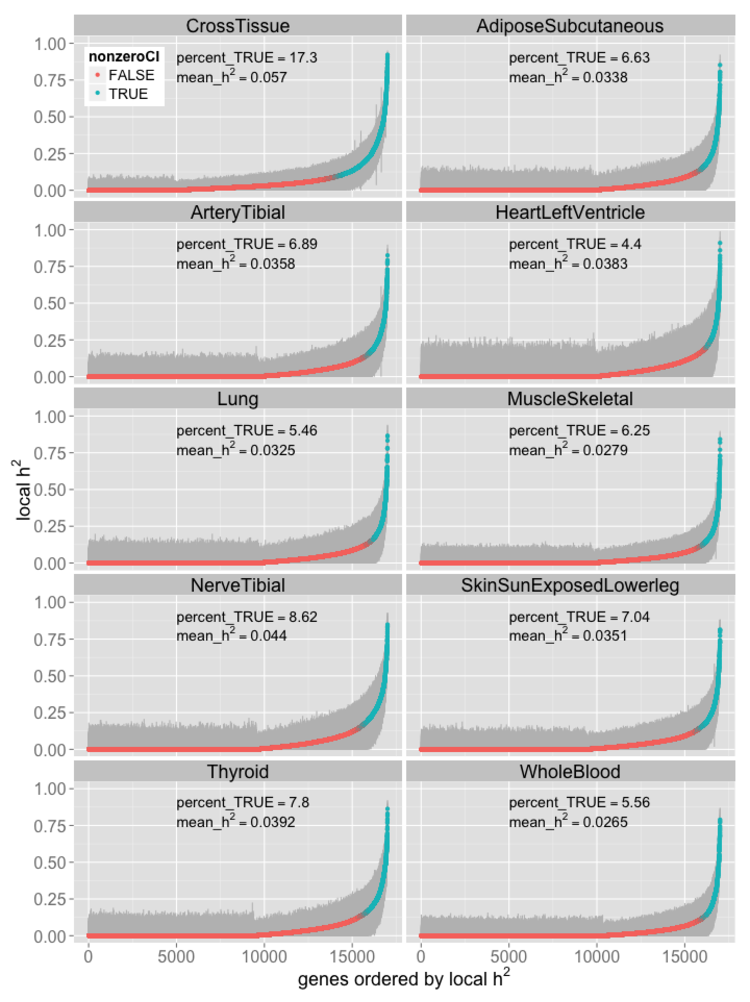
\includegraphics{GenArch_manuscript_files/figure-latex/otdTWh2-1.pdf}
\caption{Cross-tissue heritability (h\textsuperscript{2}) compared to
tissue-wide h\textsuperscript{2}. Cross-tissue local
h\textsuperscript{2} is estimated using the cross-tissue component
(random effects) of the mixed effects model for gene expression and SNPs
within 1 Mb of each gene. Tissue-wide local h\textsuperscript{2} is
estimated using the measured gene expression for each respective tissue
and SNPs within 1 Mb of each gene.}
\end{figure}

\begin{figure}[htbp]
\centering
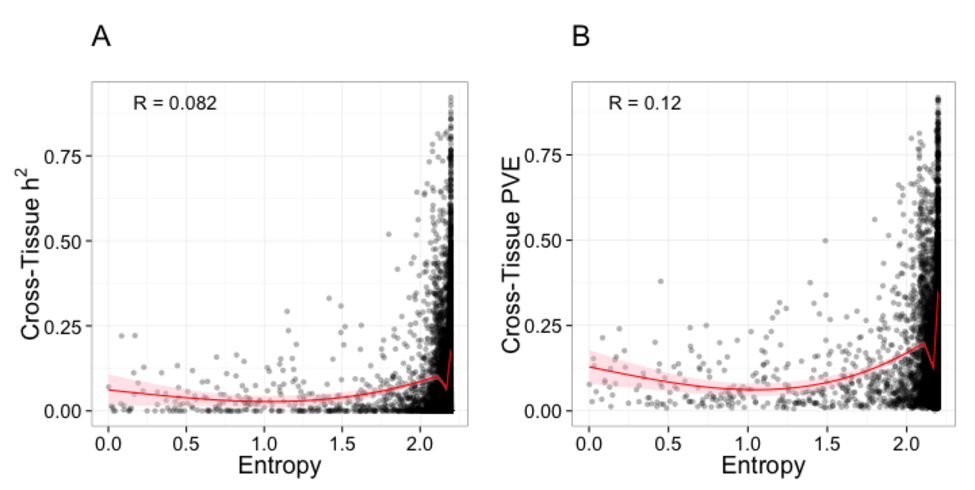
\includegraphics{GenArch_manuscript_files/figure-latex/entropyCT-1.pdf}
\caption{Entropy of the posterior probabilities from the Flutre et al.
multi-tissue eQTL method compared to the estimates of (\textbf{A})
heritability and (\textbf{B}) PVE of cross-tissue gene expression
derived from the orthogonal tissue decomposition. The generalized
additive model smoothing line is in red.}
\end{figure}

\begin{figure}[htbp]
\centering
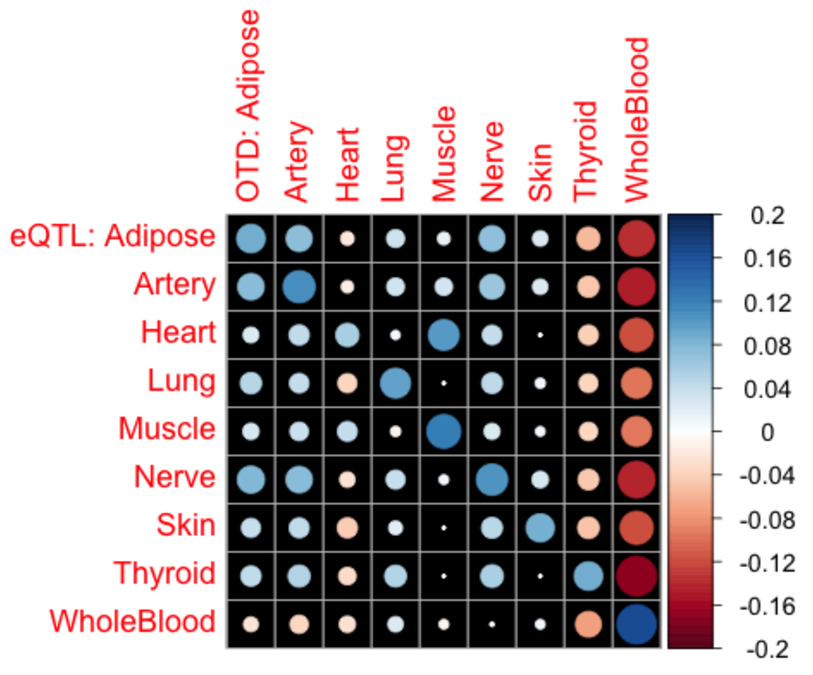
\includegraphics{GenArch_manuscript_files/figure-latex/corrplot-1.pdf}
\caption{Pearson correlation (R) between the posterior probability the
top multi-tissue eQTL regulates its gene in a given tissue (eQTL, Flutre
et al. method) and the PVE of tissue-specific gene expression from the
orthogonal tissue decomposition (OTD). Area of each circle is
proportional to the absolute value of R.}
\end{figure}

\section{Supplemental Figures}\label{supplemental-figures}

\section*{References}\label{references}
\addcontentsline{toc}{section}{References}

1. Nicolae DL, Gamazon E, Zhang W, Duan S, Dolan ME, Cox NJ.
Trait-associated SNPs are more likely to be eQTLs: Annotation to enhance
discovery from GWAS. Gibson G, editor. PLoS Genetics. Public Library of
Science (PLoS); 2010;6: e1000888.
doi:\href{http://dx.doi.org/10.1371/journal.pgen.1000888}{10.1371/journal.pgen.1000888}

2. Nica AC, Montgomery SB, Dimas AS, Stranger BE, Beazley C, Barroso I,
et al. Candidate causal regulatory effects by integration of expression
QTLs with complex trait genetic associations. Gibson G, editor. PLoS
Genetics. Public Library of Science (PLoS); 2010;6: e1000895.
doi:\href{http://dx.doi.org/10.1371/journal.pgen.1000895}{10.1371/journal.pgen.1000895}

3. Gusev A, Lee SH, Trynka G, Finucane H, Vilhj{\a'a}lmsson BJ, Xu H, et
al. Partitioning heritability of regulatory and cell-type-specific
variants across 11 common diseases. The American Journal of Human
Genetics. Elsevier BV; 2014;95: 535--552.
doi:\href{http://dx.doi.org/10.1016/j.ajhg.2014.10.004}{10.1016/j.ajhg.2014.10.004}

4. Purcell SM, Wray NR, Stone JL, Visscher PM, Sullivan MCOPF, Sklar P,
et al. Common polygenic variation contributes to risk of schizophrenia
and bipolar disorder. Nature. Nature Publishing Group; 2009;
doi:\href{http://dx.doi.org/10.1038/nature08185}{10.1038/nature08185}

5. Stahl EA, Wegmann D, Trynka G, Gutierrez-Achury J, Do R, Voight BF,
et al. Bayesian inference analyses of the polygenic architecture of
rheumatoid arthritis. Nature Genetics. Nature Publishing Group; 2012;44:
483--489. doi:\href{http://dx.doi.org/10.1038/ng.2232}{10.1038/ng.2232}

6. Morris AP, Voight BF, Teslovich TM, Ferreira T, Segr{\a`e} AV,
Steinthorsdottir V, et al. Large-scale association analysis provides
insights into the genetic architecture and pathophysiology of type 2
diabetes. Nature Genetics. Nature Publishing Group; 2012;44: 981--990.
doi:\href{http://dx.doi.org/10.1038/ng.2383}{10.1038/ng.2383}

7. Albert FW, Kruglyak L. The role of regulatory variation in complex
traits and disease. Nat Rev Genet. Nature Publishing Group; 2015;16:
197--212. doi:\href{http://dx.doi.org/10.1038/nrg3891}{10.1038/nrg3891}

8. Stranger BE, Montgomery SB, Dimas AS, Parts L, Stegle O, Ingle CE, et
al. Patterns of cis regulatory variation in diverse human populations.
Barsh GS, editor. PLoS Genetics. Public Library of Science (PLoS);
2012;8: e1002639.
doi:\href{http://dx.doi.org/10.1371/journal.pgen.1002639}{10.1371/journal.pgen.1002639}

9. Stranger BE, Nica AC, Forrest MS, Dimas A, Bird CP, Beazley C, et al.
Population genomics of human gene expression. Nature Genetics. Nature
Publishing Group; 2007;39: 1217--1224.
doi:\href{http://dx.doi.org/10.1038/ng2142}{10.1038/ng2142}

10. Innocenti F, Cooper GM, Stanaway IB, Gamazon ER, Smith JD, Mirkov S,
et al. Identification, replication, and functional fine-mapping of
expression quantitative trait loci in primary human liver tissue. Storey
JD, editor. PLoS Genetics. Public Library of Science (PLoS); 2011;7:
e1002078.
doi:\href{http://dx.doi.org/10.1371/journal.pgen.1002078}{10.1371/journal.pgen.1002078}

11. Wright FA, Sullivan PF, Brooks AI, Zou F, Sun W, Xia K, et al.
Heritability and genomics of gene expression in peripheral blood. Nature
Genetics. Nature Publishing Group; 2014;46: 430--437.
doi:\href{http://dx.doi.org/10.1038/ng.2951}{10.1038/ng.2951}

12. Price AL, Helgason A, Thorleifsson G, McCarroll SA, Kong A,
Stefansson K. Single-tissue and cross-tissue heritability of gene
expression via identity-by-descent in related or unrelated individuals.
Gibson G, editor. PLoS Genetics. Public Library of Science (PLoS);
2011;7: e1001317.
doi:\href{http://dx.doi.org/10.1371/journal.pgen.1001317}{10.1371/journal.pgen.1001317}

13. Cheung VG, Spielman RS, Ewens KG, Weber TM, Morley M, Burdick JT.
Mapping determinants of human gene expression by regional and
genome-wide association. Nature. Nature Publishing Group; 2005;437:
1365--1369.
doi:\href{http://dx.doi.org/10.1038/nature04244}{10.1038/nature04244}

14. Battle A, Mostafavi S, Zhu X, Potash JB, Weissman MM, McCormick C,
et al. Characterizing the genetic basis of transcriptome diversity
through RNA-sequencing of 922 individuals. Genome Research. Cold Spring
Harbor Laboratory Press; 2013;24: 14--24.
doi:\href{http://dx.doi.org/10.1101/gr.155192.113}{10.1101/gr.155192.113}

15. Ardlie KG, Deluca DS, Segre AV, Sullivan TJ, Young TR, Gelfand ET,
et al. The genotype-tissue expression (GTEx) pilot analysis: Multitissue
gene regulation in humans. Science. American Association for the
Advancement of Science (AAAS); 2015;348: 648--660.
doi:\href{http://dx.doi.org/10.1126/science.1262110}{10.1126/science.1262110}

16. Gamazon ER, Wheeler HE, Shah KP, Mozaffari SV, Aquino-Michaels K,
Carroll RJ, et al. A gene-based association method for mapping traits
using reference transcriptome data. Nature Genetics. Nature Publishing
Group; 2015;47: 1091--1098.
doi:\href{http://dx.doi.org/10.1038/ng.3367}{10.1038/ng.3367}

17. Regression shrinkage and selection via the lasso on jSTOR
{[}Internet{]}. \url{http://www.jstor.org/stable/2346178}; 2015.
Available: \url{http://www.jstor.org/stable/2346178}

18. Hoerl AE, Kennard RW. Ridge regression: Applications to
nonorthogonal problems. Technometrics. Informa UK Limited; 1970;12:
69--82.
doi:\href{http://dx.doi.org/10.1080/00401706.1970.10488635}{10.1080/00401706.1970.10488635}

19. {de los Campos} G, Gianola D, Allison DB. Predicting genetic
predisposition in humans: The promise of whole-genome markers. Nat Rev
Genet. Nature Publishing Group; 2010;11: 880--886.
doi:\href{http://dx.doi.org/10.1038/nrg2898}{10.1038/nrg2898}

20. Wheeler HE, Aquino-Michaels K, Gamazon ER, Trubetskoy VV, Dolan ME,
Huang RS, et al. Poly-omic prediction of complex traits: OmicKriging.
Genetic Epidemiology. Wiley-Blackwell; 2014;38: 402--415.
doi:\href{http://dx.doi.org/10.1002/gepi.21808}{10.1002/gepi.21808}

21. Zhou X, Carbonetto P, Stephens M. Polygenic modeling with bayesian
sparse linear mixed models. Visscher PM, editor. PLoS Genetics. Public
Library of Science (PLoS); 2013;9: e1003264.
doi:\href{http://dx.doi.org/10.1371/journal.pgen.1003264}{10.1371/journal.pgen.1003264}

22. Flutre T, Wen X, Pritchard J, Stephens M. A statistical framework
for joint eQTL analysis in multiple tissues. Gibson G, editor. PLoS
Genetics. Public Library of Science (PLoS); 2013;9: e1003486.
doi:\href{http://dx.doi.org/10.1371/journal.pgen.1003486}{10.1371/journal.pgen.1003486}

23. Yang J, Lee SH, Goddard ME, Visscher PM. GCTA: A tool for
genome-wide complex trait analysis. The American Journal of Human
Genetics. Elsevier BV; 2011;88: 76--82.
doi:\href{http://dx.doi.org/10.1016/j.ajhg.2010.11.011}{10.1016/j.ajhg.2010.11.011}

24. Zhang X, Joehanes R, Chen BH, Huan T, Ying S, Munson PJ, et al.
Identification of common genetic variants controlling transcript isoform
variation in human whole blood. Nature Genetics. Nature Publishing
Group; 2015;47: 345--352.
doi:\href{http://dx.doi.org/10.1038/ng.3220}{10.1038/ng.3220}

25. Zou H, Hastie T. Regularization and variable selection via the
elastic net. Journal of the Royal Statistical Society: Series B
(Statistical Methodology). Wiley-Blackwell; 2005;67: 301--320.
doi:\href{http://dx.doi.org/10.1111/j.1467-9868.2005.00503.x}{10.1111/j.1467-9868.2005.00503.x}

26. Howie B, Fuchsberger C, Stephens M, Marchini J, Abecasis GR. Fast
and accurate genotype imputation in genome-wide association studies
through pre-phasing. Nature Genetics. Nature Publishing Group; 2012;44:
955--959. doi:\href{http://dx.doi.org/10.1038/ng.2354}{10.1038/ng.2354}

27. Fuchsberger C, Abecasis GR, Hinds DA. Minimac2: Faster genotype
imputation. Bioinformatics. Oxford University Press (OUP); 2014;31:
782--784.
doi:\href{http://dx.doi.org/10.1093/bioinformatics/btu704}{10.1093/bioinformatics/btu704}

28. Harrow J, Frankish A, Gonzalez JM, Tapanari E, Diekhans M,
Kokocinski F, et al. GENCODE: The reference human genome annotation for
the ENCODE project. Genome Research. Cold Spring Harbor Laboratory
Press; 2012;22: 1760--1774.
doi:\href{http://dx.doi.org/10.1101/gr.135350.111}{10.1101/gr.135350.111}

29. Friedman J, Hastie T, Tibshirani R. Regularization paths for
generalized linear models via coordinate descent. Journal of Statistical
Software. 2010;33: 1--22. Available:
\url{http://www.jstatsoft.org/v33/i01/}

30. Simon N, Friedman J, Hastie T, Tibshirani R. Regularization paths
for cox's proportional hazards model via coordinate descent. Journal of
Statistical Software. 2011;39: 1--13. Available:
\url{http://www.jstatsoft.org/v39/i05/}

31. Zhou X, Stephens M. Genome-wide efficient mixed-model analysis for
association studies. Nature Genetics. Nature Publishing Group; 2012;44:
821--824. doi:\href{http://dx.doi.org/10.1038/ng.2310}{10.1038/ng.2310}

32. Im HK, Gamazon ER, Stark AL, Huang RS, Cox NJ, Dolan ME. Mixed
effects modeling of proliferation rates in cell-based models:
Consequence for pharmacogenomics and cancer. Akey JM, editor. PLoS
Genetics. Public Library of Science (PLoS); 2012;8: e1002525.
doi:\href{http://dx.doi.org/10.1371/journal.pgen.1002525}{10.1371/journal.pgen.1002525}

33. R Core Team. R: A language and environment for statistical computing
{[}Internet{]}. Vienna, Austria: R Foundation for Statistical Computing;
2015. Available: \url{http://www.R-project.org/}

34. Bates D, Maechler M, Bolker B, Walker S. lme4: Linear mixed-effects
models using eigen and s4 {[}Internet{]}. 2014. Available:
\url{http://CRAN.R-project.org/package=lme4}

35. Bates D, Maechler M, Bolker BM, Walker S. lme4: Linear mixed-effects
models using eigen and s4 {[}Internet{]}. 2014. Available:
\url{http://arxiv.org/abs/1406.5823}

36. Stegle O, Parts L, Piipari M, Winn J, Durbin R. Using probabilistic
estimation of expression residuals (PEER) to obtain increased power and
interpretability of gene expression analyses. Nat Protoc. Nature
Publishing Group; 2012;7: 500--507.
doi:\href{http://dx.doi.org/10.1038/nprot.2011.457}{10.1038/nprot.2011.457}

\end{document}
